For a better comparison of the learned preconditioners, the evaluations should be compared against already know working preconditioner. Because we have information about the structure of the matrices we want to precondition, that is the largest absolute value are on the diagonal and these values do  not equal to 1 or 0. Therefore a good choice of preconditioner is the Jacobi preconditioner, as mentioned in section \ref{sec: prelim precond}. This preconditioner uses the diagonal elements of a matrix as the preconditioner, \(M=diag(a_{11},a_{22},\ldots)\) for matrix \(A=(a_{i,j})\) and therefore a trivial to compute inverse. Preconditioning the test data with the Jacobi preconditioner and using this set of solver iteration counts as the point of comparison for the learned preconditioner. 

What we get from that is the Jacobi preconditioner is better than all learned preconditioners regardless of improvement function and seed, as the mean and median solver iteration count is lower for all four seeds, figure \ref{fig: initial improv test measure with jacobi}. On the individual system level comparison there are systems where the learned preconditioner has lower solver iteration counts, at most 44 systems for seed 1 and SIGN improvement function, figure \ref{fig: initial improv BvJ}. We conclude from this is that our learned preconditioner can still work, but that the current algorithm or preconditioner needs to be changed.


\begin{figure}[H]
    \center
    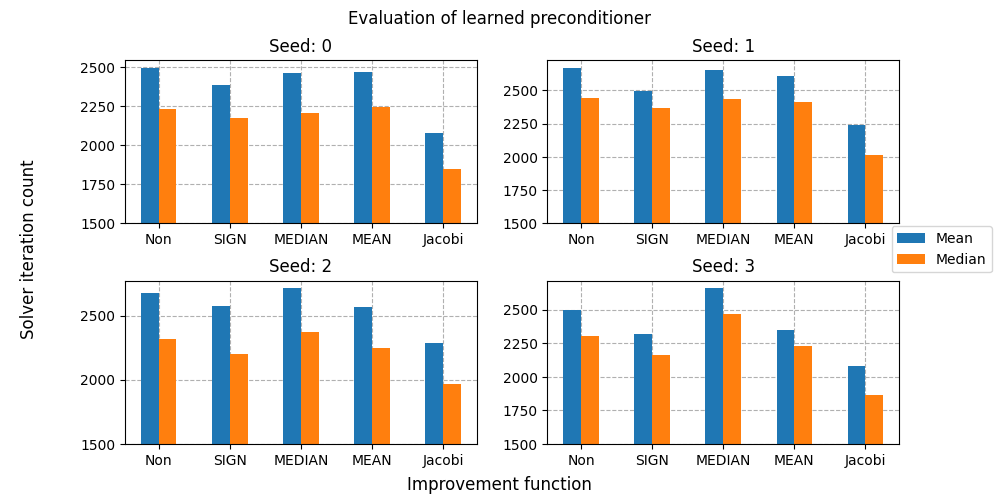
\includegraphics[width=1\textwidth]{plots/improv_func_test_measure_jacobi.png}
    \caption{The same plot as figure \ref{fig: initial improv test measure} with a bar group added for the mean and median solver iteration count for the systems preconditioned with the Jacobi preconditioner.}
    \label{fig: initial improv test measure with jacobi}
\end{figure}

\begin{figure}[H]
    \center
    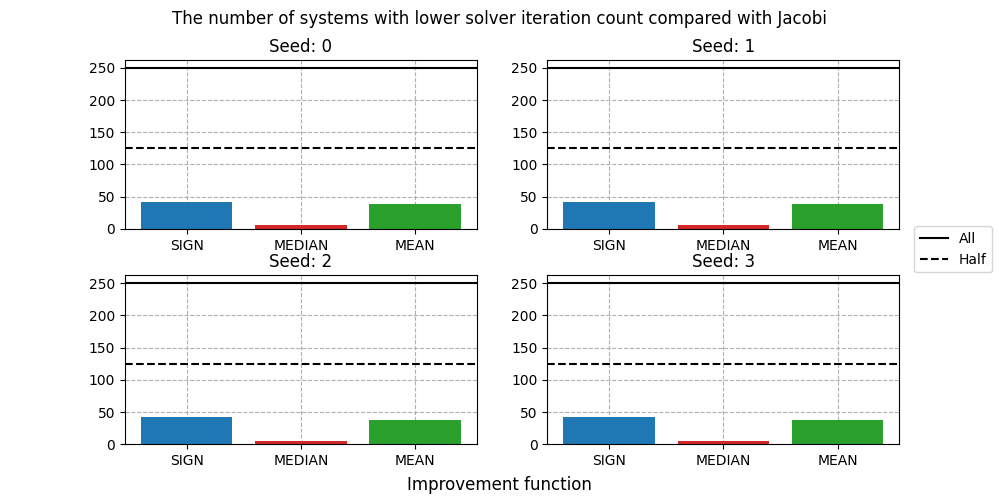
\includegraphics[width=1\textwidth]{plots/improv_func_BvJ.png}
    \caption{A similar plot to figure \ref{fig: initial improv BvN} with the difference of instead of comparing the solver iteration count to the unpreconditioned system it is compared to the systems preconditioned with Jacobi preconditioner.}
    \label{fig: initial improv BvJ}
\end{figure}

